% Sample file for AES paper

% The JAES template seems to be very old. Telling the compiler to
% use and older release of LaTeX seems to fix a bunch of errors.
% \RequirePackage[2020-02-02]{latexrelease}
\documentclass[fleqn]{jaes}

% Metadata Information
\jyear{2025}
\jmonth{April}
%\jvol{69}
%\jnum{3}

\usepackage[utf8]{inputenc}
\usepackage{amsmath}\setlength{\mathindent}{10pt}
\usepackage{bm}
\usepackage[colorlinks=false]{hyperref}
\usepackage{paralist}
\usepackage{cleveref}
\usepackage[nogroupskip]{glossaries}
\usepackage{listings}
%\usepackage{draftwatermark}
%\SetWatermarkText{DRAFT}
%\SetWatermarkColor[gray]{0.9}
%\SetWatermarkScale{1.4}
\glsdisablehyper
\newacronym{webrtc}{WebRTC}{Web Real-Time Communications}
\newacronym{mdns}{mDNS}{multicast Domain Name System}
\newacronym{daw}{DAW}{Digital Audio Workstation}
\newacronym{udp}{UDP}{User Datagram Protocol}
\newacronym{osc}{OSC}{Open Sound Control}
\newacronym{p2p}{P2P}{peer-to-peer}
\newacronym{nat}{NAT}{Network Address Translation}
\newacronym{turn}{TURN}{Traversal Using Relays around NAT}
\newacronym{stun}{STUN}{Session Traversal Utilities for NAT}
\newacronym{ice}{ICE}{Interactive Connectivity Establishment}
\newacronym{sdp}{SDP}{Session Description Protocol}
\newacronym{cgnat}{CGNAT}{Carrier-Grade Network Address Translators}
\newacronym{ip}{IP}{Internet Protocol}
\newacronym{rtp}{RTP}{Real-time Transport Protocol}
\newacronym{dtls}{DTLS}{Datagram Transport Layer Security}
\newacronym{sctp}{SCTP}{Stream Control Transmission}
\newacronym{mtu}{MTU}{Maximum Transmission Unit}
\newacronym{lan}{LAN}{Local Area Network}
\newacronym{sim}{SIM}{Subscriber Identity Module}
\newacronym{vpn}{VPN}{Virtual Private Network}
\newacronym{w3c}{W3C}{World Wide Web Consortium}
\newacronym{gbps}{Gbps}{Gigabits Per Second}
\newacronym{qos}{QoS}{Quality of Service}
\newacronym{url}{URL}{Uniform Resource Locator}
\newacronym{kks}{KKS}{The Knowledge Foundation}
\newacronym{isp}{ISP}{Internet Service Provider}
\newacronym{rush}{RUSH}{Reliable (Unreliable) Streaming Protocol}
\newacronym{iot}{IoT}{Internet of Things}
\newacronym{iresap}{IRESAP}{Information Retrieval in Embedded Systems for Audiovisual Artistic Processes}

\usepackage{xcolor}
\newcommand{\daniel}[1]{\textcolor{cyan}{[DH: #1]}} %Daniel's comments
\newcommand{\dhsuggestion}[1]{\textcolor{blue}{[DH Suggestion: #1]}} %Daniel's comments


% \makeglossaries

\lstdefinestyle{codestyle}{
    numberstyle=\tiny,
    basicstyle=\ttfamily\scriptsize,
    breakatwhitespace=false,         
    breaklines=true,                 
    captionpos=b,                    
    keepspaces=true,                 
    numbers=left,                    
    numbersep=5pt,                  
    showspaces=false,                
    showstringspaces=false,
    showtabs=false,                  
    tabsize=2
}
\lstset{style=codestyle}
\crefname{lstlisting}{listing}{listings}
\Crefname{lstlisting}{Listing}{Listings}

\begin{document}

% Page heads
\markboth{FRANKLIN ET AL.}{Development of a Web-Based Real-Time Distributed Reverberation Chamber for Live Concert Applications}

% Title portion
\title{Development of a Web-Based Real-Time Distributed Reverberation Chamber for Live Concert Applications\thanks{Correspondence should be addressed to Austin franklin}}

%Author Info.
\authorgroup{
\author{AUSTIN FRANKLIN,\textsuperscript{1,2}}
\author{RICHARD MITIC,\textsuperscript{1}}
\author{DANIEL HEDIN,\textsuperscript{1,4}}
\author{RIKARD LINDELL,\textsuperscript{3,1}}
AND \author{HENRIK FRISK,\textsuperscript{2}}
\email{(austin.franklin@mdu.se)\quad(richard.mitic@mdu.se)\quad(daniel.hedin@mdu.se)\quad(rli@du.se)\quad(henrik.frisk@kmh.se)}
\affil{\textsuperscript{1}School of Innovation, Design, and Technology, Mälardalen University, Västerås, Sweden \\
\textsuperscript{2}Department of Composition, Conducting, and Music Theory, The Royal College of Music, Stockholm, Sweden \\
\textsuperscript{3}Dalarna Audiovisual Academy (DAVA), Dalarna University, Falun, Sweden \\
\textsuperscript{4}Department of Computer Science and Engineering, Chalmers University of Technology, Gothenburg, Sweden}
}

%Abstract
\abstract{%
This paper documents the challenges encountered during the development of a mobile web-based, real-time distributed reverberation chamber for a live concert setting. Initial efforts focused on leveraging existing open source and commercial solutions, but these proved inadequate due to limitations in network compatibility, audio routing, and mobile device support. WebRTC emerged as the most viable option, offering peer-to-peer communication and firewall traversal capabilities. However, significant obstacles persisted, including network reliability, audio hardware/software ecosystem limitations, and debugging complexity. The project highlights the fragmented nature of real-time audio streaming technologies and the need for more transparent, reliable, and well-documented tools. Despite these challenges, we developed a functional web application prototype using WebRTC, Web Audio API, and custom session description protocol modifications, offering insights into the complexities of deploying real-time audio systems over mobile networks. The paper concludes with reflections on speculative approaches, such as decentralized audio routing and native app development, and calls for improved documentation and standardized debugging tools to support future innovations.
}

\maketitle

%Head 1
\section{INTRODUCTION}
We began a project in February 2024 to create a simple proof-of-concept: distributing a live reverberation chamber as a stereo audio signal over a mobile network from a concert hall to up to three (3) remote locations, and back to the original site, where an audience would experience the distributed performance alongside a live music event. The end goal was to create a merged reality for the audience and to explore their experience of the site-specific aural qualities of the remote locations merged with those of the concert hall. The prototype, named Auxtrument, was officially used in concert in November 2024 following a successful demonstration at the 2024 International Conference on Quality of Multimedia Experience (QoMEX'24) \cite{franklin2024merging}.

We anticipated that this project would be a relatively straightforward endeavor, given the established use of network-based tools for collaborative performance. We initially explored available open-source and commercial solutions, but each proved inadequate for various reasons. Our efforts extended to experimenting with various protocols and network stacks, leading us to settle on \gls{webrtc} as the most viable option. \gls{webrtc} is marketed as a reliable, standardized solution that appeared to address the core challenges we faced: seamless real-time communication across devices, browsers, and networks \cite{loreto_real-time_2014}. However, even after adopting \gls{webrtc}, significant obstacles persisted, particularly in three key areas: \begin{inparaenum}[1)] \item network compatibility and stability, \item limitations within the audio hardware and software ecosystem, and \item debugging complexity and software fragmentation\end{inparaenum}. Many of these challenges remained unresolved throughout the project, contradicting \Glspl{webrtc} reputation as a mature and reliable technology.

Boem et al. state that platforms based on \gls{webrtc} were not originally designed for networked music experiences but rather as `environments where a single data stream... is broadcast to all users simultaneously' \cite{nime2024_33}. Additionally, they suggest that overcoming these limitations using custom servers and protocols, while possible, remains challenging. These issues raise critical questions about the reliability, scalability, and practical limitations of these tools--where things like frequent version updates and deprecations can be difficult to track across multiple web stacks and may render software components, or even entire applications, unusable. While the Auxtrument application provided a workable solution, the development and testing process exposed significant gaps in documentation, unpredictable `black box' network behaviors, and difficulties in achieving consistent performance across different devices and environments.

\begin{figure*}
    \centering
    
\includegraphics[width=0.99\linewidth]{tools.png}
    \caption{The timeline of development for the Auxtrument.}
    \label{fig:tools}
\end{figure*}

\Cref{fig:tools} shows our development. Each item represents a tool, protocol, or software/hardware component laid out in the order in which we experimented with it. Given the aims and timeline of the project, we did not conduct a proper state-of-the-art investigation into the full gamut of mobile web audio streaming technologies. Given the reputation of \gls{webrtc} as tried-and-tested software, and the saturation of open-source and commercially available audio streaming solutions, it was not reasonable for us to assume that many of the problems we encountered were not already solved. Instead, we document our journey, highlighting our motivations and processes, aiming to shed light on the broader complexities of deploying real-time audio systems over mobile networks using exploratory and practice-based methods.

\section{METHODOLOGY}
Exploratory research, as described by Stebbins, emphasizes open-ended investigation into uncharted territories, allowing us to document and reflect on unexpected outcomes during the process \cite{astebbins_exploratory_2001}. We also apply practice-based research methods, in which creative practice serves as both the process and outcome of research, generating new insights through artistic exploration and critical reflection \cite{candy_practice_2006,scrivener_art_2002}. To distinguish our work as practice-based, we structured the methodology to align with the criteria proposed by Scrivener \cite{scrivener_art_2002}:

\begin{enumerate}
    \item Define the objectives and research question(s).
    \item Document the tools, setup, and actions used.
    \item Analyse the results, noting the challenges.
\end{enumerate}

Our research began with an artistic question: \textit{How can the real-time distribution of site-specific acoustic reverberation between a concert hall and multiple remote locations create a merged reality audience experience?} However, as development progressed, we encountered a series of challenges--including network reliability, limitations in existing audio ecosystems, and debugging complexities--and our focus necessarily shifted. In response, the research question evolved: \textit{What are the practical and technical constraints of implementing a mobile, real-time, distributed reverberation system for live performance using existing audio streaming technologies?}

To investigate this question, we established three (3) objectives for achieving a high-fidelity user experience: 1) the audio signals must be high-resolution to preserve the inherent quality of the transmitted sounds and accurately relay spatial properties of the acoustic environments; 2) the system should be easy to set up and use, and work over different types of networks; and 3) to support use in any location, it must be compatible with mobile devices. This framing allowed us to critically assess available tools and infrastructures as active conditions that shape the artistic possibilities of the original research question. In writing this paper, we set out to retroactively analyse and better understand the causes behind several of these challenges. We document our findings here in the belief that they contribute to a broader understanding of how current technologies shape the possibilities--and limits--of mobile networked music performance, while also illuminating the assumptions embedded in their design and use.

\section{SURVEY OF TECHNOLOGIES}
In evaluating potential software solutions, we conducted hands-on tests with a variety of audio applications, focusing primarily on their networking capabilities and suitability for real-time audio transmission of multiple channels and audio routing capabilities across different platforms and clients. Given the goal of integrating mobile devices with the Auxtrument, we also explored applications with mobile support. However, we did not test mixer apps on mobile phones, as these typically require custom plugins for advanced routing and signal processing--something that mobile operating systems restrict. As we are primarily composers, sound artists, and researchers, we explored solutions well-known in our respective field(s), and the list of software is by no means exhaustive. These findings guided our decision to further explore alternative networking approaches for real-time audio streaming.

\subsection{EXISTING AUDIO APPLICATIONS}
Though our aim was to have Auxtrument work on mobile networks, our initial tests involved using JackTrip \cite{noauthor_jack_2024} and SonoBus \cite{noauthor_sonobus_2024} on MacBook laptops. We started with laptops and Wi-Fi connections, anticipating this would be a quick and practical first step in prototyping while allowing us to evaluate the software. Although JackTrip’s user interface was straightforward, it lacked the flexibility we needed for audio routing between clients, sending the same audio stream to all participants without the ability to control volume or mute channels on the host side. It also did not have an implementation for mobile phones. These limitations made it unsuitable for our purposes. SonoBus, on the other hand, addressed this issue by offering a mobile app and multichannel input/output capabilities, allowing users to specify channel destinations.

We attempted to connect using SonoBus over a mobile hotspot using the Swedish Tele2 service provider, with one laptop connected via eduroam. Eduroam is a global network roaming service for students and employees in academia \cite{wierenga_eduroam_2015}. Its authentication requirements are standardized across all networks, but individual providers can and often add additional security features. The setup using SonoBus with Tele2 and eduroam proved unsuccessful. In contrast, connections between two laptops granted eduroam certificates worked, and even certified mobile devices connected to eduroam were able to stream audio via the SonoBus iOS app without issues.

These initial findings led us to suspect that the security features implemented at Mälardalen University and The Royal College of Music in Stockholm, where eduroam networks are accessible, were blocking \gls{p2p} connections from external networks. A major obstacle was SonoBus's lack of options to specify ports or other network settings, making it ineffective when dealing with firewall restrictions. This posed a significant obstacle, as eduroam was our primary testing network, and we had no reliable way to determine in advance whether an external network would permit a connection. 

\Glspl{daw} are powerful tools that feature a wide range of audio plugins. Reaper \cite{noauthor_reaper_nodate} and Logic \cite{noauthor_logic_nodate} can host Apple’s AUNetSend and AUNetReceive plugins which are used to send audio between applications, hardware instruments, and more on a Mac \cite{noauthor_audio_nodate}. However, these plugins use zero-configuration networking through Bonjour \cite{noauthor_bonjour_nodate} and \gls{mdns} service records to send audio over a \gls{lan} only. Other well established live audio tools such as Cycling ‘74 Max have networking capabilities, limited primarily to control data via \gls{udp} and \gls{osc} protocols \cite{amo2014max}. One workaround for audio streaming is to convert audio vectors to jitter matrices and send the video stream over the network. However, Max is not compatible with iOS.

Following the completion of the prototype, we broadened our search of existing audio streaming applications. We found the Virtual Rehearsal Room (VRR) and a list of alternatives \cite{vrr_alternatives}. VRR is based on Audio over OSC (AoO), the underlying protocol behind SonoBus, using Pure Data as a plug-in for the Mozilla browser \cite{ritsch2014towards}. These alternatives--including LoLa, NinJam, and Soundjack--reflect a range of design priorities and technical trade-offs. LoLa, for example, requires dedicated hardware and a stable one (1) \gls{gbps} connection, typically only available on academic networks. While \glspl{isp} advertise such speeds, real-world performance varies. NinJam, bundled with Reaper, addresses latency by aligning performers to musical measures, sometimes increasing latency by one or more bars. Soundjack uses \gls{p2p} networking but requires \gls{udp} port 50050 to be forwarded--an issue on networks like eduroam, where port forwarding is often blocked for security reasons.

What became clear through this review was that no single tool fit our needs perfectly. SonoBus remains the closest to meeting our criteria due to its cross-platform support and intuitive interface. Yet the inability to manually configure network ports or tunnel through more restrictive firewalls ultimately limited its utility in real-world settings. As a final thought, the process of evaluating these alternatives confirmed that while the existing ecosystem of remote audio tools is mature in some respects, it remains fragmented, with little attention paid to mobile-first, multi-endpoint collaboration under institutional network conditions.

\subsection{EXISTING WEB TECHNOLOGIES}
To create a realistic reverberation chamber effect, minimizing network latency was essential. Although we did not set a strict target, our goal was to reduce the delay below the threshold of the precedence effect of approximately 40ms for complex sounds such as speech and music \cite{wallach1949precedence}. Beyond this threshold, the delayed sound is perceived as a distinct echo rather than a single auditory event. Given this requirement, it was determined that \gls{p2p} connections would be the most suitable approach.

We explored existing technologies and protocols. For instance, we made an implementation that relies on WebSockets through Node.js by setting up a remote server and having clients connect to a central computer. Our assumption was that WebSockets, being a well-established technology, would provide a reliable foundation for audio transmission. However, we quickly encountered a significant challenge--WebSockets by themselves were unable to reliably connect two devices on disparate networks. Given these limitations, we eventually decided that building a mobile web app using \gls{webrtc} would be the most feasible approach due to its native \gls{p2p} and firewall traversal capabilities and broad browser support.

\gls{webrtc} relies on the clients negotiating a suitable way to connect to each other. The process of negotiation, known as signaling, takes place outside the \gls{webrtc} framework, e.g., using a custom built signaling server based on WebSockets. The first step exchanges session descriptions in the form of a \gls{sdp} offer that describes the type of connection (if it is video or audio), the codecs and codec parameters to be used, and more. The second step of signaling uses \gls{ice} to establish a way for the peers to stream to each other.

\gls{ice} looks for the lowest latency connection by trying to 1) establish a \gls{p2p} connection using a \gls{stun} or \gls{turn} server, 2) establish a direct TCP connection via the HTTP and HTTPS ports, and 3) falling back on an indirect connection via a \gls{turn} server. This means that even in cases where \gls{nat} prohibits a \gls{p2p} connection using STUN, the TURN relay should act as a failsafe that permits the connection, albeit with increased overall latency, provided that it is explicitly configured to do so.

\section{THE AUXTRUMENT AND THE NETWORK}
From an implementation perspective, the final version of the Auxtrument is a web application based on \gls{webrtc} that is deployed using Express.js \cite{noauthor_express_nodate} running on top of Node.js \cite{noauthor_nodejs_nodate}. The Peer.js library is used for establishing the connection \cite{noauthor_peerjs_nodate}. Peer.js is a free library and service intended to provide easy-to-use \gls{webrtc} connections. On the client side it provides a library that wraps \gls{webrtc}, allowing clients to establish connections using only an ID. This requires the use of a Peer.js signaling server that uses the IDs to automate the connection process. Peer.js provides its own signaling servers and the source code for the server to enable projects to host their own applications. 

This stack helps streamline and simplify the number of actions a user must perform to establish a connection. Users simply navigate to the \gls{url} and select whether they are the central hub or location peers. The signaling and \gls{p2p} initiation is automatically handled in the background, and the audio input and output devices are specified by each client in the user interface prior to establishing a connection. The concert-ready version of the Auxtrument is limited to three remote clients and one central hub but nothing prevents further expansion into more complex configurations.

\subsection{NETWORK CHALLENGES}
Due to the limited number of IPv4 addresses, most \Glspl{isp} rely on some form of \gls{nat} or \gls{cgnat}. This allows multiple clients to share the same external \gls{ip} address, thus conserving the address space. \gls{nat} and \gls{cgnat} typically prevent connections to clients to be initiatiated from the outside, which causes problems if two peers situated behind \gls{nat} or \gls{cgnat} want to establish \gls{p2p} connections. Similar situations may occur when firewalls are used to protect local networks. The first priority of the \gls{ice} protocol is to find ways to establish \gls{p2p} connections in the presence of \gls{nat}, \gls{cgnat} or firewalls, e.g., using `hole punching.' Somewhat simplified, hole punching is based on indirectly manipulating the state of the firewall or NAT by initiating communication from the inside of a network in such a way that the initiator is exposed on the external network \cite{ford2005peer}.

Experiments with the Auxtrument show the complexity of the network setup and identifying and mediating issues. Tests with Tele2 and Tre for example, some of Sweden's largest mobile service providers, did not work with our \gls{webrtc} implementation whatsoever using STUN. Because of the fact that most of our testing occurred between eduroam networks, where we are based, and other \Glspl{isp}, it was not immediately apparent that the mobile network itself, or combination of \gls{isp} and eduroam networks together, was the problem over firewall restrictions when used with laptops.

This led to tests with other mobile network providers in Sweden, primarily by visiting service provider stores, setting up some basic equipment, and running the Auxtrument using borrowed \glspl{sim}. Based on these tests, we discovered that Telia worked perfectly in all the situations where other providers previously had not. The frustration with mobile network providers is that there is no way to know exactly why Telia works and the others do not, in terms of how specifically each \gls{cgnat} is configured, and what penetration methods might be successful prior to experimentation. To complicate the matter further, we were able to get a connection working behind \gls{cgnat}, but via a fibre-based \gls{isp}.

We experimented with exploring the networks using traceroute, but the results were inconclusive. While there are other tools for mapping the architecture of a network, we did not pursue them due to the complexity of the setup, in particular the interaction between the \gls{ip} layer and the mobile network that, among other things, allows for roaming between carriers. As Kanaris and Pouwelse note, there are many different network configurations and \gls{nat} architectures that make penetration techniques difficult. However, they document an issue where both peers behind the same \gls{cgnat} cannot establish a connection using \gls{stun} since the server is outside of the intranet and only sees the `middle' network \cite{kanaris2023mass}. This explains, at least in part, some of our issues when testing with Tele2 mobile networks.

\subsection{WEBRTC MEDIA STREAM}
\gls{webrtc} presented challenges with minimising latency using its adaptive jitter buffer. The buffer automatically resizes when latency exceeds its capacity and does not reset unless the web page is refreshed. Setting the jitter buffer is `best effort,' meaning that \gls{webrtc} may not honor the request and prioritize its own settings in cases where there are network interruptions. There are other not-so-well known methods for minimising latency, such as implementing a playout delay--a \gls{rtp} header extension, which provides the sender’s intent to the receiver on how quickly a frame needs to be rendered \cite{schulzrinne2003rfc3550}. Community forums and bug reports show mixed reviews with playout delay implementation, with some suggesting the feature does not work with Chrome’s Javascript API layer at all. This mirrors our experience using this feature in Chrome.

\subsection{WEBRTC DATA CHANNEL}
We explored using the \gls{webrtc} Data Channel to overcome latency issues and have explicit control over the jitter buffer. By sending segments of audio data as bytes via this channel, we hoped to piggyback on its low latency performance and then create an audio channel for playback on the other end. Initially, the latency was acceptable for our use case, between 10-40ms, however, it would unexpectedly increase to around 20-30 seconds for brief moments of time. When this occurred the audio was significantly affected, with clear indications of data loss. We were initially astonished: Where do those packets live for such a long time? While we have been unable to reproduce the issue in a controlled manner, it seems to be easier to trigger on unreliable networks (i.e., mobile networks).

We hypothesise that it is a combination of network \gls{qos} and \Glspl{webrtc} use of \gls{sctp} for reliable data channel messaging \cite{stewart2022rfc}. Specifically, when a transmitted message exceeds the \gls{mtu} of the network, it is segmented into smaller portions. Variable latency in each segment can be due to scheduling messages in the network stack, congestion, or differing processing times between network nodes, and this latency can easily compound. When packets arrive out of order, additional buffering, reordering mechanisms, or even retransmission may be needed. Even though the channel can be configured to be `unordered' to reduce latency, lost packages still need to be retransmitted to preserve audio quality. It could be the case that high network congestion causes frequent retransmission, further exacerbating the congestion and data loss. We assume \gls{qos} plays a part in this process since \Glspl{webrtc} media stream does not suffer from the same issue. Furthermore, there are unknowns about the ways in which mobile network topology contributes to latency, given that some tests with 5G encountered greater variance, while 4G seemed to provide more reliable results.

Moreover, when implementing our own jitter buffer using the data channel, we discovered an unexpected issue where playback sounded like white noise rather than the intended audio stream, even when testing using a \gls{lan}. The issue occurred when the buffer size grew too large, with the exact threshold depending on the mobile device's browser running the node client. Strangely, setting the buffer past this threshold caused the client to misinterpret the type of data, specified as frames of 128 bytes, from an \texttt{ArrayBuffer} to an \texttt{UInt8Array}, causing the audio data to be in the range of 0 to 255 instead of the intended normalised range of -1 to 1. The \gls{webrtc} data channel effectively supports dynamic typing through Javascript, but it's not explicitly defined by the API itself. Instead, the data type is dynamically determined at runtime based on what is passed to \texttt{send()}, and the receiver must handle different types accordingly. We have no explanation as to why this process fails in our own implementation using the data channel.

\section{THE AUXTRUMENT AND AUDIO}
The Auxtrument uses the open-source and royalty free Opus codec that is preferred by \gls{webrtc} \cite{valin2012rfc}. It operates with a sampling rate of 48 kHz to match that of most web browsers to prevent resampling at any stage in the transmission process, along with variable bitrate encoding. The recording for both the locations and the central hub is handled using the web browsers’ \texttt{get\-UserMedia()} javascript function of the MediaDevices API, which returns an audio stream from the selected audio input device.

At the same time, audio playback requires the Web Audio API. Once the audio has been received from all locations, the hub parses the channels from the streams of each location and merges them into a single multi-channel stream. For instance, three (3) locations with three (3) interleaved stereo streams are merged into a single stream with six (6) channels that is sent to a multi-channel audio device and controlled via a mixer (\Cref{fig:audio}). This process is performed using the splitter and merger web audio graph nodes \cite{noauthor_web_audio}. The splitter transforms the interleaved stereo signals into separate mono signals, and then the merger node mixes all (6) mono signals for the left and right channels, respectively.

\begin{figure*}
    \centering
    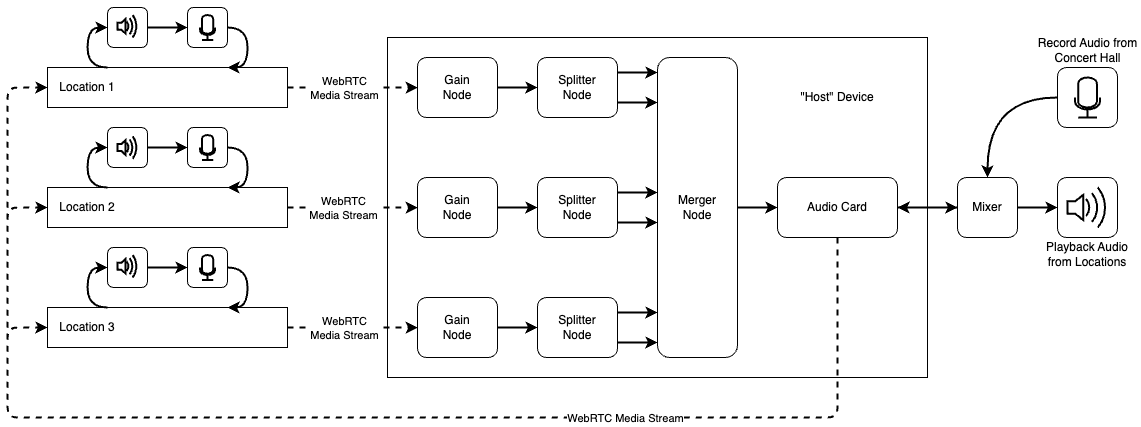
\includegraphics[width=0.99\linewidth]{audio.png}
    \caption{WebRTC and Web Audio API between Auxtrument peers.}
    \label{fig:audio}
\end{figure*}

\subsection{WEBRTC \Gls{sdp}}
When setting up the aforementioned \gls{webrtc} connection, the protocol requires stream configuration information. \gls{sdp} munging is required to configure a media stream to contain more than the default single channel \cite{begen_sdp_2021}. The \gls{sdp} is the standard that describes media communication sessions, and it contains the codec parameters, source address, and timing information of audio and video streams. For the Auxtrument, streaming stereo audio--to be diffused in the concert hall--was chosen as the minimum requirement for achieving an immersive experience, while remaining lightweight enough to minimize hardware demands and avoid potential bandwidth issues. Using \gls{webrtc}, streaming a stereo signal requires forcing the boolean \texttt{stereo=1} flag to the description. However, the \gls{webrtc} documentation makes no mention of editing the \gls{sdp} or specifying stereo transmission, and in hindsight, this makes sense given that most \gls{webrtc} applications use mono audio streaming for video conferencing.

In addition to this, \glspl{webrtc} \texttt{getUserMedia()} function includes a \texttt{channelCount} constraint that allows users to specify the number of channels in the local stream. This does not, however, determine the number of channels you are expecting to send and be received by another peer over the network. That property must be munged in the \gls{sdp} file negotiated between two peers during signaling. Without this, a stereo signal is taken from one peer and a mono signal is received by the other. For multichannel audio specifically, the required codec name is \texttt{multiopus} as opposed to \texttt{opus}, which also must be munged in the \gls{sdp} offer along with the channel configurations. However, \gls{webrtc} does not mention the codec, and in both cases, the necessary solutions were found in community forums. \Cref{lst:sdp} shows a function that edits the \gls{sdp} file for multichannel streaming.

\begin{figure}[h!]
\begin{lstlisting}[caption=SDP munging function, label=lst:sdp]
function modifySDPForStereo(sdp) {
  const sdpLines = sdp.split('\r\n');
    for (let i = 0; i < sdpLines.length; i++) {
      if (sdpLines[i].startsWith('a=fmtp:111')) {
        sdpLines[i] += 'channel_mapping=0,1,2,3,4,5';
        num_streams=4;coupled_streams=2;
        maxaveragebitrate=510000';
      }
      if (sdpLines[i].startsWith('a=rtpmap:111')) {
        sdpLines[i] = 'a=rtpmap:111 multiopus/48000/6';
      }
    }
  const modifiedSDP = sdpLines.join('\n');
  return modifiedSDP;
}
\end{lstlisting}
\end{figure}

\subsection{AUDIO ECOSYSTEM LIMITATIONS}
To ensure ease of use and portability, we prioritized mobile device support--enabling connections from remote locations with minimal hardware while maintaining reliable connections. We focused on iOS development primarily because most of our team uses Apple devices. Apple's restrictive approach to external microphone compatibility is part of its broader sandboxing and security philosophy, which prioritizes system integrity over user flexibility. While this makes iOS more secure and stable, it also creates significant challenges for real-time audio applications--especially those relying on \gls{webrtc} and web-based tools rather than native apps \cite{blochberger2019state}. Unlike macOS, where \gls{webrtc} freely accesses external audio devices via standard APIs, iOS restricts audio input at the system level. Even when a device is selected using \Glspl{webrtc} input selection function, iOS does not always honor the selection. This was the case with a Zoom ZMS-44 2-channel audio interface, which promised iOS compatibility.

After testing other devices, the R\O DE NTG mobile boom mic proved compatible with Google Chrome and \gls{webrtc} on iOS. However, iOS treated the external mic as an additional input rather than a full replacement. The internal mic did not turn off completely and continued picking up audio, albeit at a lower volume. The streams for both inputs were merged into a single channel and sent over the network, leading to an undesirable mix of sources. In the end, our investigation ended here--mainly due to time constraints--however, the R\O DE NTG proved otherwise successful given our project goals. The R\O DE NTG also features a 3.5mm line output that was used with an OB-1 speaker by Teenage Engineering for playback.

\section{DEBUGGING}
While developing the Auxtrument in line with our objectives, we encountered numerous challenges and gained valuable insights. However, debugging proved particularly difficult due to the complex and fragmented nature of the technology stack, which involved multiple layers and components. Furthermore, the lack of comprehensive and accurate documentation often hindered our progress, forcing us to rely on community forums and other unofficial sources.

\subsection{DEBUGGING COMPLEXITY}
Debugging presented a huge challenge throughout the project, particularly because of the `black box' nature of these technologies and the fact that hearing no sound from another location during testing could represent one of dozens of potential issues, many of which are extremely time consuming, if not impossible to find. Problems could lie with audio hardware, operating system, browser type and version, \gls{webrtc}, Web Audio API, our own implementation, a library, or mobile network(s). In most browsers, for example, \gls{webrtc} and Web Audio API work together seamlessly, whereas in latest version of Safari at the time (17.5.1), multi-channel through the Web Audio API became non-functional after updating.

Furthermore, a known regression in Safari 17.5.1 causes the \texttt{AudioContext()} to stop after the browser loses and then regains focus (e.g., minimizing the window) \cite{WebKitBug276016}. Even when interacting with UI elements designed to produce sound, the audio remains unresponsive for the rest of the session. This is indicative of broader challenges with WebKit, the engine underlying Safari, which has historically lagged in implementing certain web standards. For instance, the \texttt{AudioWorklet} interface, crucial for low-level audio processing, was not implemented in WebKit until 2021, hindering developers relying on this feature for enhanced audio capabilities \cite{MDNAudioWorkletNode}. These inconsistencies across the Apple ecosystem add complexity to debugging, as behaviors can vary significantly between WebKit and other browser engines and devices, sometimes necessitating browser-specific workarounds.

Another major challenge is logging and monitoring in a real-time \gls{webrtc} environment. Traditional in-browser debugging tools often fall short because \gls{webrtc} operates asynchronously and across multiple layers, meaning errors can occur at any stage--signaling, negotiation, network transport, or playback--without clear visibility into where the failure originates. While tools like \texttt{webrtc-internals} (Chrome) and \texttt{about:webrtc} (Firefox) can provide useful insights, they require detailed expertise to interpret, and they don’t always reveal the full picture when dealing with custom audio routing or multi-channel implementations. They also do not communicate any information about how, if at all, \gls{webrtc} and Web Audio API are collaborating.

The abstraction process used by Peer.js makes establishing connections across devices and networks easier, but more difficult to control and debug. For instance, there are bug reports that express difficulty connecting certain mobile providers. There are even reports with Peer.js and iOS version compatibility, suggesting it is not guaranteed to work across all variations reliably. Furthermore, Peer.js includes its own list of STUN and TURN servers to use as defaults. In many reports, mirrored by our own experience, the Peer.js TURN relay tries repeatedly to negotiate between candidates before eventually failing to establish a connection. As a post concert test, we set up our own TURN relay through Metered, a WebRTC TURN relay service, and noticed a bug in the Auxtrument code that was not properly overwriting the default Peer.js servers with our own server specifications. After fixing the issue, we were able to establish a connection using our TURN relay on both eduroam and Tele2 networks. This points to an issue with the TURN relays provided by Peer.js.

One reason we did not suspect Peer.js sooner was because it does not log anything, and we had no reason to expect that our servers were not even being considered. When we began development, we explicitly decided against using a TURN relay due to its added latency (an average roundtrip time of approximately 115 ms based on some of our tests). It's possible that considering this option sooner, rather than for trying to debug network issues after the fact, might have helped us discover the problem with Peer.js earlier in the development process. In any case, this says nothing about the use of STUN with different network architectures and \Glspl{nat}, which still presents significant challenges.

\subsection{DOCUMENTATION}
There were many moments throughout development where a property, method, or constraint was not documented through the \Glspl{webrtc} documentation repository. Instead, these were found elsewhere on community forums such as Stack Overflow, CodePen examples, and Reddit threads. A recent Editor’s Draft from \gls{w3c} that was published on the 13th of February 2025 includes the most complete overview of the more esoteric capabilities of \gls{webrtc} that we have been able to find \cite{jennings_webrtc_nodate}.

Although this is an incomplete draft as of the day of this publication, many unknowns about \gls{webrtc} features are revealed, although the information is largely inaccurate. For example, the \texttt{channelCount} constraint is initially listed as a boolean, but another place on the same Web page correctly lists it as unsigned long. This is the case with all constraints \gls{webrtc} describes in this draft. The latest published version from 8th of October 2024 makes one mention of the \texttt{channelCount} constraint, but does not define it or reference how it should be used and with what data type.

\section{OTHER APPROACHES}
There are several speculative approaches and improvements that could have been considered to answer our research question and address the challenges presented in this paper. While \gls{webrtc} provided a workable solution, the unpredictability of its implementation and distribution, particularly for a live concert setting, highlights the need for more user friendly and reliable solutions.

\subsection{DECENTRALIZED AUDIO ROUTING}
Instead of relying on a single \gls{webrtc}-based application to handle all connections, we could have used separate devices for each pair of connections. This approach would have simplified the network topology and reduced the complexity of debugging, as each connection would be independent. However, this would have required more devices. Although we chose to develop a web-based application for its cross-platform compatibility, we could have considered developing a native app for iOS and Android. A native app would have provided better access to device hardware and operating system features, custom handling of jitter buffers, and compensation for packet losses, thus potentially overcoming some of the limitations presented using web-based solutions.

\subsection{VIRTUAL PRIVATE NETWORKS}
Routing all connections over a \gls{vpn} could have simplified peer discovery since each device can be assigned a hostname or static virtual \gls{ip} address. We decided against this option in practice simply because the \gls{webrtc} application was already developed. We also posited that the underlying network routes of a \gls{vpn} would effectively be the same as those negotiated by \Glspl{webrtc} \gls{ice} protocol and therefore the \gls{vpn} would serve no additional benefit. However, the \Glspl{vpn} data encryption may slightly increase overall transmission latency.

As a retrospective test, we attempted to recreate the Auxtrument between two SonoBus clients connected to a \gls{vpn}--a laptop connected to a corporate WiFi network, and an iPhone connected to the Tre mobile network. Using SonoBus' \textit{connect to group} functionality the laptop connected successfully. When the phone attempted to connect, an error message appeared and no audio was transferred. Using SonoBus' experimental \textit{direct connection} functionality using the \glspl{ip} provided by the \gls{vpn}, we were only able to send audio in one direction--from phone to laptop. There was no further debugging information available from SonoBus so it is unclear exactly where the error occurred.

\subsection{ALTERNATIVE PROTOCOLS}
As a potential alternative to \gls{webrtc}, we experimented with creating a transmission protocol similar to \gls{rush} \cite{pugin_rush_2021}, which is based on QUIC \cite{iyengar_quic_2021} and allows fine-grain control over delivery guarantees and avoidance of congestion. However, it was determined that implementing an entire streaming protocol from scratch was not feasible in the time available. One of the marketed benefits of \gls{webrtc} was that the implementation already exists in browsers, and for a networked music performance we were inclined to favour tried-and-tested software over an experimental option.

%% Due to formatting this text does not fit unless I remove the \break command before the bios section which AES may not like. I shortened my bio but it doesn't help. Neither did it help to remove the "Vision" section and put the text into CONCLUSIONS. I think the best is to keep it short and just hope they accept it. Or remove it.

\section{OUR VISION}
The grand vision of the research project (IRESAP) is the ambition to have a musical performance in a remote locations where the performers and the audience are interconnected through a mobile interface. This interface will allow access not only to the sound of the performance but to the data involved in producing the performance, thereby blurring the performer-audience boundary. In addition, we also envision participants coming and going from the performance ecosystem in real-time. Currently, \gls{iot} technologies are the only viable option for such a system, placing great importance on established technologies such as \gls{webrtc}. This vision could, for example, be an merged reality concert where the functionality of the Auxtrument allows any user to filter sound through the physical environment of another user at any time. For this--and other experimental network music performance applications--to succeed, the technologies discussed in this paper need to be reliable, robust, and scalable.

% 
%If there was a piece of software that was already doing, which we thought, this we would have used it

%What's the vision long term, why is this important/useful 

%Even though systems for networked performance, the liberty of performing music at various locations on mobile networks without latency should be a game changer for the field of music production.
%% its all about time, as soon you have latancey and time critical.

\section{CONCLUSION}
One of the primary challenges we faced was the lack of comprehensive documentation for \gls{webrtc}, especially multi-channel audio and \gls{sdp} munging. In the future, we would expect more detailed and accessible documentation for developers. In addition, we hope for the development of standardized debugging tools that provide better visibility into the interaction between \gls{webrtc} and Web Audio API in the browser. \gls{webrtc} has been available since 2011 and stable since 2018. Nevertheless, we suggest that web browser developers increase their efforts to make their implementations compliant with \gls{w3c} standards. Finally, addressing the issues with mobile networks regarding transparency and compatibility are paramount, particularly with STUN server signaling, but also wishful thinking. Perhaps until the transition to IPv6 address space is complete, or until NAT vendors become more aware of the requirements of significant \gls{p2p} applications, many of these mobile network challenges will remain unsolved.

Our journey creating a web-based, real-time distributed reverberation chamber reveals both the potential and limitations of current technologies for real-time audio streaming over mobile networks. While \gls{webrtc} provided a foundational solution, its implementation exposed significant challenges, including network compatibility issues, and hardware/software ecosystem limitations, and debugging complexity. These challenges highlight the need for more robust, transparent, and well-documented tools to support real-time audio applications. Looking ahead, the development of standardized debugging tools and more comprehensive documentation for \gls{webrtc} and related technologies will be critical for advancing real-time audio streaming applications. This project serves as a case study in the complexities of web audio technologies and offers valuable insights for future research and development.

\section{ACKNOWLEDGMENTS}
\gls{iresap} is supported by \gls{kks}.

% - If you are using bibTex for references, you need these lines: 
% \bibliography{jaes.bib}
\bibliography{auxtrument}
\bibliographystyle{jaes.bst}

%\break

%\printglossary[title=GLOSSARY]

%Biography
\biography{Austin franklin}{austin.jpg}{Austin Franklin is a composer and researcher at Mälardalen University and the Royal College of Music in Stockholm, working with information retrieval, embedded systems, and artistic processes. He maintains a real-time timbral analysis library for Cycling '74 Max. His music has been performed at Carnegie Hall and received awards including the American Prize and the Petrichor International Music Competition.
}

\biography{Richard Mitic}{richard.jpg}{Richard Mitic is a PhD candidate at Mälardalen University, researching spatial audio, digital signal processing, and large-scale music information retrieval. He holds a master's in Music and Electronics from the University of Glasgow and has extensive industry experience--from working with media streaming protocols and MPEG standardization to software for music streaming.%Richard Mitic is a PhD candidate at Mälardalen University researching spatial audio, digital signal processing, and large-scale music information retrieval. He holds a masters degree in Music and Electronics from the University of Glasgow where he specialized in digital electronics and audio processing. He has spent many years in industry, starting as a researcher of media streaming protocols and participating in MPEG standardization, later progressing into the music industry where he wrote software for music streaming, media transcoding, real-time audio, and embedded devices.
}
 
\biography{Daniel Hedin}{daniel.png}{Daniel Hedin is a senior lecturer in computer science at Mälardalen University and a guest researcher at Chalmers University of Technology, specializing in language-based security. His research covers secure information flow, data minimization, and formal verification, with a recent focus on securing untrusted code and web applications. He is the principal designer of several practical tools, including JavaScript sandboxes and security-enhanced interpreters.%Daniel Hedin is a senior lecturer in computer science at Mälardalen University and a long-term guest researcher at Chalmers University of Technology focusing on language-based security. His research interests include static and dynamic analysis of security properties of programs, secure information flow and data minimization as well as formal modeling and proofs of security of systems. Recently, his research has focused on secure execution of untrusted code and enforcement of secure information flow in the setting of web applications. He is the principal designer of several practical security tools, including JavaScript sandboxes and security-enhanced interpreters.
}

\biography{Rikard Lindell}{rikard.jpg}{Rikard Lindell is a composer and professor at Mälardalen University (computer science, interaction design) and Dalarna University (audiovisual studies). His artistic work includes interactive installations, electroacoustic and orchestral compositions, and phonogram releases. In research, he explores code as design material and contributes to the NIME community. He has developed commercial audiovisual performance apps for iOS.%Rikard Lindell is a composer of electronic music, experience designer, code artisan, associate professor in computer science with focus on interaction design and Mälardalen University, and professor in audiovisual studies at Dalarna University. As an artist he has exhibited several interactive sound and light installations, composed electric music and music for orchestra, and participated on several phonograms. In research he has contributed in code as design material and in the community of new interfaces for musical expressions. He has also developed commercial audiovisual performance apps for the iOS platform.
}
 
\biography{Henrik Frisk}{henrik.jpg}{Henrik Frisk is a composer and performer of contemporary music. He is a professor of composition at the Royal College of Music in Stockholm, where he teaches electroacoustic music. His research focuses on improvisation, interactivity, spatialisation, and experimental music, with current projects exploring spatial perception and multidisciplinary approaches to electronic music heritage.%Henrik Frisk is an active performer (saxophones and electronics) and composer of contemporary music. He is professor of music, teaching composition at the department for electroacoustic music at the ´Royal College of Music in Stockholm. His research is concerned with improvisation, interactivity, spatialisation, method development, and experimental electroacoustic music. Currently involved in several projects, including studies in the perception of spatiality and a project employing multidisciplinary approaches to electronic music heritage, his research focuses mainly on artistic practices. 
}

\end{document}
